\documentclass[UTF8]{ctexart}
\usepackage{graphicx}
\usepackage{amsmath}
\usepackage{bibentry,natbib}
\usepackage{fancyhdr}

\title{The theory in Word2Vec}
\author{BrightHush}
\date{\today}

\begin{document}
\maketitle
\tableofcontents

\pagestyle{fancy}
\cfoot{\thepage}

\newcommand{\figref}[1]{\figurename~\ref{#1}}

\section{Introduction}
Word2Vec中实现了两个模型,分别是CBOW(Continuous Bag of Words)模型和Skip-gram模型。
CBOW模型,在训练过程中是指给出了当前词的上下文,预测出现当前词的概率,其模型架构如图\ref{Fig:CBOW}。
而Sikp-gram模型,则是在给定当前词的情况下,计算上下文出现的概率,该模型可参见\ref{Fig:skipgram}。
\begin{figure}[h!]
    \centering     
    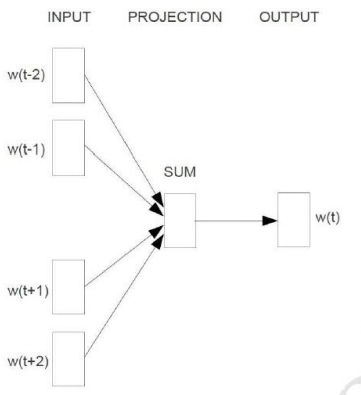
\includegraphics[width=0.5\textwidth]{cbow}   
    \caption{\label{Fig:CBOW}CBOW Architecture} 
\end{figure}

\begin{figure}[h!]
    \centering     
    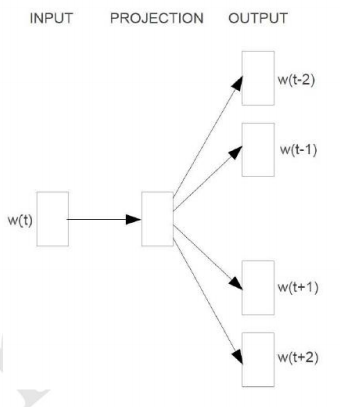
\includegraphics[width=0.5\textwidth]{skipgram}   
    \caption{\label{Fig:skipgram}Skip-gram Architecture} 
\end{figure}

\par
在word2vec中,分别基于 Hierarchical Softmax 和 Negative Sampling 的方法进行建模,下面的note
会详细讨论CBOW和Skip-gram在这两个方法下的细节。
\par
根据语言模型的定义,通常是给定上下文求出现下一个词的概率,基于这样的思路,在神经网络概率语言模型中,
我们也是需要建立这样的条件概率模型。因此COBW和Sikp-gram的log似然可以分别表示为(\ref{cobw-likelihood})
和(\ref{skipgram-likelihood})。
\begin{align}
\label{cobw-likelihood}
L &= \sum_{w \in C} log(P(w|Context(w)))
\\
\label{skipgram-likelihood}
L &= \sum_{w \in C} log(P(Context(w) | w)) 
\end{align}

\par
下面的讨论将会将重点放在如何构建这个条件概率上,这也是使用 Hierarchical Softmax 和 Negative Sampling 的
本质区别所在。

\section{Hierarchical Softmax}
由于Bengio在06年提出的Neural Network Language Model训练时间主要耗费在输出层的Softmax上,因此
Hierarchical Softmax 方法,是通过在神经网络的输出层加上一个二叉树来减少 NNLM 在输出层的计算量。下面
将分别针对 COBW 和 Skip-gram 展开讨论模型的构建细节。

\subsection{CBOW with Hierarchical Softmax}
首先来看看该模型的网络结构,如果对于当前词w和其对应的上下文Context(w),可表示为如图\ref{Fig:cbow-hs} ,
分为以下三层:
\begin{itemize}
\item[输入层]:输入层为词w对应上下文词所对应的词向量,也就是该词前c个词和后c个词,分别将词映射到对应的向量。
\item[投影层]:投影层仅仅是将输入层的各个词对应的词向量进行相加,得到$X_w$。
\item[输出层]:输出层对应一个二叉树,在Word2Vec则是按照词频构建一棵哈夫曼树。二叉树的叶子节点对应词典中的
每个词,非叶子节点则可以看成是一个二类Logistic分类器。
\end{itemize}
\begin{figure}[h!]
    \centering     
    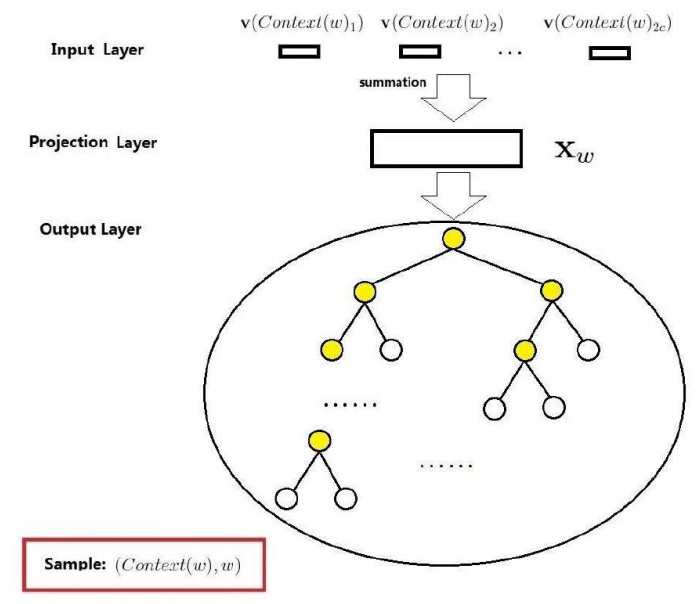
\includegraphics[width=1.0\textwidth]{cbow-hs}   
    \caption{\label{Fig:cbow-hs}CBOW with Hierarchical Softmax} 
\end{figure}

\par
在 Hierarchical Softmax 中,词汇表中的每个词对应二叉树中的一个叶子节点,从根节点到叶子节点的路径是确定的。
如果说把每一个非叶子节点看成是一个分类器,那么这个二叉树就相当于一个决策树,根据从根节点到叶子节点的路径,我们可以
计算在输入$X_w$的情况下的对应叶子节点对应词的条件概率,也就是我们上面希望建模的 Language Model 。
\par
对于一个训练样本,我们记当前词为w,那么我们需要说明如下的符号:
\begin{itemize}
\item[1.] $p^w$表示从根节点到w对应叶子节点的路径;
\item[2.] $l^w$表示路径$p^w$对应的节点个数;
\item[3.] $p_j^w(j \in [1, l^w])$表示路径$p^w$中的第j个节点;
\item[4.] $d_j^w(j \in [2, l^w])$表示路径中第j个节点对应的编码,对应值为0或者1,根节点不对应编码;
\item[5.] $\theta_j^w(j \in [1, l^w-1])$表示路径中第j个节点对应Logistic分类器参数,
          叶子节点并不产生分类,所以不对应$\theta$参数。
\end{itemize}
\par
在 Huffman Tree 的每个节点进行分类的时候,我们按照Logistic Classification的思路,每个非叶子节点
对应一个$\theta$参数,于是在该节点上输入被分类为正类的概率可表示为:
\[ \sigma(x_w^T \theta) = \frac{1}{1 + e^{-x_w^T \theta}} \]
那么该节点上被分为负类的概率则为:
\[ 1 - \sigma(x_w^T\theta)\]
word2vec中将编码为1的定义为负类,编码为0的定义为正类,其实这里的编码为0或者1,取决于在构造Huffman Tree
的时候,你怎么定义。在word2vec中,将两个兄弟节点中较小的编号为1。

\par
在训练样本中,给定一个(w, Context(w)),那么我们在投影层计算得到$x_w$之后,进入到输出层,也就是进入到
Huffman Tree 的结构中。这个时候,从根节点走到w对应叶子节点的过程中,共经历了$l^w-1$次分类,那么由
Context(w) 得到 w 的条件概率可以表示为:
\begin{equation}
\label{cbow-hs}
p(w|Context(w)) = \Pi_{j=2}^{l^w} p(d_j^w|x_w, \theta_{j-1}^w)
\end{equation}
那么对应的条件概率根据其在 Huffman Tree 上的编码确定
\begin{equation}
p(d_j^w|x_w, \theta_{j-1}^w)= \begin{cases}
\sigma(x_w^T \theta_{j-1}^w), \quad d_j^w=0
\\
1 - \sigma(x_w^T \theta_{j-1}^w), \quad d_j^w=1
\end{cases}
\end{equation}
按照 Logistic Regression 中的方式将上面的分段函数写在一起则可以表示为:
\[ p(d_j^w|x_w, \theta_{j-1}^w) = (\sigma(x_w^T \theta_{j-1}^w))^{1-d_j^w} %
\cdot (1-\sigma(x_w^T\theta_{j-1}^w))^{d_j^w} \]
\par
综合上式和(\ref{cbow-hs}),将其代入到(\ref{cobw-likelihood})中,我们可以得到log似然表示为:
\begin{align}
L &= \sum_{w \in C} log \Pi_{j=2}^{l^w}p(d_j^w|x_w, \theta_{j-1}^w)
\\
&= \sum_{w \in C} \sum_{j=2}^{l^w} \left( (1-d_j^w)log(\sigma(x_w^T \theta_{j-1}^w)) %
+ d_j^w log(1-\sigma(x_w^T\theta_{j-1}^w)) \right)
\end{align}
\par
为了推导计算梯度方便,我们记上式大圆括号中的内容为
\begin{align}
L(w, j) = (1-d_j^w)log(\sigma(x_w^T \theta_{j-1}^w)) + d_j^w log(1-\sigma(x_w^T\theta_{j-1}^w))
\end{align}
\par
上式中,我们只有两个参数$(x_w, \theta_{j-1}^w)$,我们将$L(w, j)$对这两个参数进行求偏导,那么我们
可以得到下面的两个梯度计算公式:
\begin{align}
\frac{\partial L(w, j)}{\partial \theta_{j-1}^w} &= %
(1 - d_j^w - \sigma(x_w^T \theta_{j-1}^w))x_w
\\
\frac{\partial L(w, j)}{\partial x_w} &= %
(1 - d_j^w - \sigma(x_w^T \theta_{j-1}^w))\theta_{j-1}^w
\end{align}
于是$\theta_{j-1}^w$的更新公式可以表示为:
\[ \theta_{j-1}^w := \theta_{j-1}^w + \eta (1 - d_j^w - \sigma(x_w^T \theta_{j-1}^w))x_w \]
而对于词对应的词向量应该如何更新呢?我们计算的是$L(w, j)$对$x_w$的偏导,而$x_w$为Context(w)
中的词向量之和,所以\[ \frac{\partial L(w,j)}{\partial v_u} = %
\frac{\partial L(w,j)}{\partial x_w} \frac{\partial x_w}{\partial v_u} \quad u \in Context(w)\]
其中$v_u$表示词$u$对应的词向量,于是词向量对应的更新方式如下:
\[ v_u := v_u + \eta \sum_{j=2}^{l^w} (1 - d_j^w - \sigma(x_w^T \theta_{j-1}^w))\theta_{j-1}^w %
\quad u \in Context(w) \]
其中$v_w$表示词w对应的词向量。


\subsection{Skip-gram Architecture}
对于 Skip-gram 模型,其构建思路是希望在已知w的情况下,预测Context(w)的情况。Skip-gram的结构如图\ref{Fig:skip-hs}。
\begin{figure}[h!]
    \centering     
    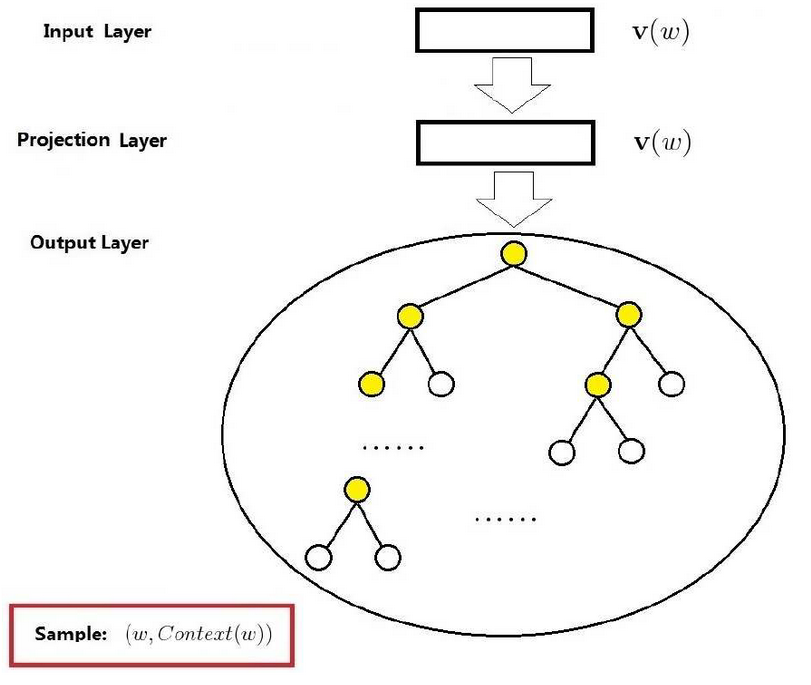
\includegraphics[width=1.0\textwidth]{skipgram-hs}   
    \caption{\label{Fig:skip-hs}Skip-gram with Hierarchical Softmax} 
\end{figure}
此时的输入层为词w对应的当个词向量,投影层不做任何操作,只是为了讨论的统一。输出层同CBOW模型一样,是一棵二叉树,
叶子节点对应每个词,非叶子节点可以理解为二分类器,参数为$\theta$。
\par
根据Skip-gram的思想,希望通过当前词预测上下文的思路,并且根据(\ref{skipgram-likelihood})我们可以构建
条件概率的计算方法为:
\begin{align}
p(Context(w)|w) &= \Pi_{u \in Context(w)} p(u|w) 
\\
p(u|w) &= \Pi_{j=2}^{l^u} p(d_j^u|v_w, \theta_{j-1}^u)
\\
p(d_j^u|v_w, \theta_{j-1}^u) &= \theta(v_w^T \theta_{j-1}^u)^{1-d_j^u} %
(1-\theta(v_w^T)\theta_{j-1}^u)^{d_j^u}
\end{align}

\par
那么对于训练数据集C的log似然可以表示为如下:
\begin{align}
L &= log \Pi_{w \in C} \Pi_{u \in Context(w)} \Pi_{j=2}^{l^u} %
p(d_j^u|v_w, \theta_{j-1}^u)
\\
&= \sum_{w \in C} \sum_{u \in Context(w)} \sum_{j=2}^{l^u} %
log p(d_j^u|v_w, \theta_{j-1}^u)
\\
&= \sum_{w \in C} \sum_{u \in Context(w)} \sum_{j=2}^{l^u} %
(1-d_j^u)log(\theta(v_w^T \theta_{j-1}^u)) + %
d_j^u log(1 - \theta(v_w^T \theta_{j-1}^u))
\end{align}
为了下面描述梯度计算的方便,我们将上式三重求和符号内部的式子表示为
\[L(w, u, j) = (1-d_j^u)log(\theta(v_w^T \theta_{j-1}^u)) + %
d_j^u log(1 - \theta(v_w^T \theta_{j-1}^u)) \]
对上式分别对参数$v_w$和$\theta_{j-1}^u$进行求偏导可得:
\begin{align}
\frac{\partial L(w, u, j)}{\partial \theta_{j-1}^u} &= %
(1 - d_j^u - \theta_{j-1}^u)v_w
\\
\frac{\partial L(w, u, j)}{\partial v_w} &= %
(1 - d_j^u - \theta_{j-1}^u)\theta_{j-1}^u
\end{align}
梯度更新的时候就需要注意了,按照随机梯度下降的思路,如果是把一个(w, Context(w))当成是一个
sample的话。那么$v_w$的梯度上升大小肯定是$\sum_{u \in Context(w)} \sum_{j=2}^{l^u} L(w, u, j)$
的所有对$v_w$有梯度计算的梯度之和,而对于$\theta_{j-1}^u$,由于Context(w)中包含多个词,那么从根
到叶子节点的路径上可能重复某个非叶子节点,那么这个时候的$\theta_{j-1}^u$与$\theta_{j'-1}^{u'}$很有
可能是同一个中间节点,那么对这个节点的$\theta$的梯度就应该是各个单独梯度之和了。上述的两个更新方式,是严格按照
$\sum_{u \in Context(w)} \sum_{j=2}^{l^u} L(w, u, j)$这个来的,也是随机梯度下降的时候需要注意的。


\section{Negative Sampling}
Negative Sampling 与 Hierarchical Softmax 方法不同之处在于如何构造(\ref{cobw-likelihood})
和(\ref{skipgram-likelihood})两个条件概率。HS方法通过在网络的输出层构造一棵二叉树,从根节点走到
对应叶子节点表示一个概率。而在Negative Sampling方法中,每个词有一个$\theta$参数,直接用这个参数估计
在给定输入情况下,该词出现的概率,这个概率的计算使用Logistc Classification的方法。整个模型构造完成之后,
目标函数仍然定义为训练语料的Language Model表示的似然,这个Language Model可以是
CBOW,也可以是Sikp-gram。有了目标函数之后,使用梯度上升法来最大化这个似然,求解的参数是$(\theta, v_w)$。
\par
现在问题来了,我们似乎是在训练在某个输入下,某个词出现的概率,其实就是对应该词的一次分类,那么问题来了,我们在给定
(w, Context(w))或者(Context(w), w)中,我们只有正样本,那么我们如何生成正样本呢?这就是Negative Sampling
名称的由来。
\par
以(w, Context(w))为例,在对应$(w, u)\quad u\in Context(w)$时,我们把u当成$\theta^u$的正样本,然后
从词典中随机几个非u的词作为负样本,u的负样本集合我们表示为$NEG_u$,于是我们对当前这个(w, u)的似然表示为
\[ L(w, u) = p(1|v_w, \theta^u) \Pi_{u' \in NEG_u}(1-p(1|v_w, \theta^{u'}))\],其中
\[ p(1|v_w, \theta^u) = \sigma(v_w^T\theta^u)\],也就是Logistic Classification中分为正样本的概率。
\par
通过上述对Negative Sampling算法描述,可以知道该算法是非常快速的算法。Hierarchical Softmax算法对于一个样本的计算
复杂度取决于从根节点到叶子节点路径的长度,而对于Negative Sampling中,仅仅取决于我们希望Sample 多少个负样本,因此
Negative Sampling是非常快的算法。

\section{Summarize}
其实Language Model就相当于一个分类问题,一个词代表一个类别,只不过这个类别非常的多。于是最初的Neural Network Language
Model使用的是Softmax作为神经网络的最后一层,在这个基础上,很多工作都是希望加速这个训练过程。于是出现了
Hierarchical Softmax 和 Negative Sampling,这两个方法都是基于分类的思想来加速 word vector 训练过程。
这两个模型本身并不复杂,但是能想到用这种方式来训练word vector就是一个非常大的创新,事实上也得到了不错的效果。
跳出原有的思维模式,换一种思路来解决问题,在改变问题定义的同时使用某种程度上的近似,从而达到近似求解原问题的目的,
这样的创新是值得我们学习的。

\section{References}
\begin{itemize}
\item[1] word2vec 中的数学原理详解, \\
\url{http://blog.csdn.net/itplus/article/details/37969519}.
\end{itemize}

\end{document}
